% PNAS website: https://www.pnas.org/page/authors/submission

% Only a single PDF file containing all text, figures, tables, and supporting information (SI) is required for initial submissions; high-resolution files are not required.

% The preferred length of articles is 6 pages, but PNAS will allow articles up to a maximum of 12 pages.

% Proof pages - Word count - Maximum no. of figures and tables - Maximum no. of references
% 6   4,000   4   50
% 7   4,500   5   55
% 8   5,000   6   60
% 9   5,500   7   70
% 10  6,000   8   75
% 11  6,500   9   80
% 12  7,000   10  85

% Include department, institution, and complete address, with the ZIP/postal code, for each author. Use lower case letters to match authors with institutions, as shown in the example. Authors with an ORCID ID may supply this information at submission.

% All authors must submit their articles at http://www.pnascentral.org/cgi-bin/main.plex. If you are using Overleaf to write your article, you can use the ``Submit to PNAS'' option in the top bar of the editor window.

% Images must be provided at final size, preferably 1 column width (8.7cm). Figures wider than 1 column should be sized to 11.4cm or 17.8cm wide. Numbers, letters, and symbols should be no smaller than 6 points (2mm) and no larger than 12 points (6mm) after reduction and must be consistent. 

% Authors should submit SI as a single separate SI Appendix PDF file, combining all text, figures, tables, movie legends, and SI references. PNAS will publish SI uncomposed, as the authors have provided it. Additional details can be found here: https://www.pnas.org/page/authors/format#Supporting_Information. Refer to the SI Appendix in the manuscript at an appropriate point in the text. Number supporting figures and tables starting with S1, S2, etc.

% Use the lineno option to display guide line numbers if required.
\documentclass[9pt,twocolumn,twoside,lineno]{pnas-new}

% other packages
\usepackage{xspace}

% self-defined commands
\newcommand{\degreesC}{\textdegree C\xspace}
\newcommand{\degrees}{\textdegree\xspace}
\newcommand{\dC}{$\delta^{13}$C\xspace}
\newcommand{\dO}{$\delta^{18}$O\xspace}
\newcommand{\SrSr}{$^{87}$Sr/$^{86}$Sr\xspace}
\newcommand{\OsOs}{$^{187}$Os/$^{188}$Os\xspace}
\newcommand{\permil}{\textperthousand\xspace}
\newcommand{\pCOtwo}{\textit{p}CO$_{2}$\xspace}
\newcommand{\COtwo}{CO$_{2}$\xspace}

\templatetype{pnasresearcharticle}

\title{Emergence of the Southeast Asian islands as a driver for Neogene cooling}

% Use letters for affiliations, numbers to show equal authorship (if applicable) and to indicate the corresponding author
\author[a,1]{Yuem Park}
\author[a]{Pierre Maffre} 
\author[b]{Yves Godd\'eris}
\author[c]{Francis A. Macdonald}
\author[c]{Eliel A. Anttila}
\author[a]{Nicholas L. Swanson-Hysell}

\affil[a]{Department of Earth and Planetary Science, University of California, Berkeley, CA 94720, USA}
\affil[b]{G\'eosciences Environnement Toulouse, CNRS--Universit\'e Paul Sabatier - IRD, Toulouse 31400, France}
\affil[c]{Department of Earth Science, University of California, Santa Barbara, CA 93106, USA}

% Please give the surname of the lead author for the running footer
\leadauthor{Park} 

% Authors must submit a 120-word maximum statement about the significance of their research paper written at a level understandable to an undergraduate educated scientist outside their field of speciality. The primary goal of the significance statement is to explain the relevance of the work in broad context to a broad readership. The significance statement appears in the paper itself and is required for all research papers.
\significancestatement{Authors must submit a 120-word maximum statement about the significance of their research paper written at a level understandable to an undergraduate educated scientist outside their field of speciality. The primary goal of the significance statement is to explain the relevance of the work in broad context to a broad readership. The significance statement appears in the paper itself and is required for all research papers.}

% Please include corresponding author, author contribution and author declaration information
\authorcontributions{Please provide details of author contributions here.}
\authordeclaration{No competing interests to declare.}
\correspondingauthor{\textsuperscript{1}To whom correspondence should be addressed. E-mail: yuempark@berkeley.edu}

% At least three keywords are required at submission. Please provide three to five keywords, separated by the pipe symbol.
\keywords{Keyword 1 $|$ Keyword 2 $|$ Keyword 3 $|$ ...} 

% Please provide an abstract of no more than 250 words in a single paragraph. Abstracts should explain to the general reader the major contributions of the article. References in the abstract must be cited in full within the abstract itself and cited in the text.
\begin{abstract}
The steep topography, tropical climate, and mafic lithologies of the Southeast Asian islands contribute to efficient chemical weathering and carbon sequestration. Concurrent with global cooling since the mid-Miocene, ongoing collision between the Sunda-Banda arc and Australia has increased the area of subaerially-exposed land in the region. Here we integrate lithology into a coupled weathering-climate model to assess how the global climate system responds to changes in paleogeography. We then use paleoshoreline data as boundary conditions to quantify the change in steady-state \pCOtwo associated with the tectonic emergence of the Southeast Asian islands since the mid-Miocene. We find that the modeled decrease in \pCOtwo due to these paleogeographic changes is sufficient to explain long-term climatic cooling over the Neogene.
\end{abstract}

\dates{This manuscript was compiled on \today}
\doi{\url{www.pnas.org/cgi/doi/10.1073/pnas.XXXXXXXXXX}}

\begin{document}

\maketitle
\thispagestyle{firststyle}
\ifthenelse{\boolean{shortarticle}}{\ifthenelse{\boolean{singlecolumn}}{\abscontentformatted}{\abscontent}}{}

\dropcap{T}he Southeast Asian islands (SEAI) have an out-sized contribution to modern chemical weathering fluxes. The confluence of steep topography, a warm and wet tropical climate, and the presence of mafic lithologies results in high fluxes of Ca and Mg cations and associated \COtwo consumption \cite{Gaillardet1999a}. There has been a significant increase of subaerially-exposed land area within the region since the Miocene associated with ongoing arc-continent collision between Australia and the Sunda-Banda arc system \cite{Molnar2015a, Macdonald2019a}. Concurrently, after the Miocene Climatic Optimum, a cooling trend began ca. 15~Ma and accelerated over the past 4 million years (m.y.) culminating with the onset of Northern Hemisphere glaciation \cite{Zachos2008a}. Many hypotheses have been proposed to explain this cooling trend including changes in ocean/atmosphere circulation \cite{Haug1998a, Shevenell2004a, Molnar2015a}, a decrease in volcanic outgassing \cite{Berner1983a}, or uplift in the Himalaya \cite{Raymo1992a, Galy2007a}. Here we instead propose that SEAI emergence was itself sufficient to explain long-term climatic cooling over the Neogene.

Over geologic time-scales, \COtwo enters Earth's ocean--atmosphere system primarily via volcanism and metamorphic degassing, and leaves primarily through the chemical weathering of silicate rocks, with a smaller sink through organic carbon burial \cite{Kump1997a}. Chemical weathering delivers alkalinity and cations to the ocean which drives carbon sequestration through carbonate precipitation. Steady-state \pCOtwo is set at the \pCOtwo level at which \COtwo sinks are equal to sources. As \COtwo sinks are removed and \pCOtwo rises, temperature increases and the hydrological cycle is invigorated, causing other weathering sinks to increase until a new steady-state is achieved at higher \pCOtwo \cite{Kump1997a}. Conversely, as regions with high carbon sequestration potential emerge on Earth's surface, \pCOtwo decreases resulting in other weathering sinks to diminish leading to a new lower steady-state \pCOtwo concentration.

Topography, climate, and lithology all effect chemical weathering. High-relief regions lead to reaction-limited weathering regimes that are more sensitive to climate change \cite{Gabet2009a, West2012a}. In warm and wet regions, mineral dissolution kinetics are faster leading to enhanced chemical weathering \cite{West2012a}. Mafic rocks have higher Ca and Mg concentrations and dissolution rates than felsic rocks, and thus the potential to more efficiently sequester carbon through silicate weathering \cite{Dessert2003a}. These factors have lead to the proposal that arc-continent collisions within the tropical rain belt have been important in enhancing global weatherability, lowering atmospheric \pCOtwo, and initiating glacial climate over the past 520~m.y. \cite{Jagoutz2016a, Swanson-Hysell2017a, Macdonald2019a} and perhaps in the Neoproterozoic as well \cite{Park2019b}.

To estimate the decrease in steady-state \pCOtwo associated with the increase of subaerially-exposed land area in SEAI, we use the global spatially-resolved GEOCLIM model \cite{Godderis2017c}. GEOCLIM estimates changes in steady-state \pCOtwo associated with coupled changes in chemical weathering and climatology by linking a silicate weathering model to climate model runs at multiple \pCOtwo levels.

The silicate weathering component of GEOCLIM calculates \COtwo consumption resulting from silicate weathering for subaerially-exposed land. In previous versions of the model, silicate weathering was a function of temperature and runoff only, and all bedrock was assigned identical chemical compositions \cite{Godderis2017c}. More recent versions of GEOCLIM implement regolith development and soil shielding, which introduces a dependence on erosion (and therefore topographic slope) \cite{Maffre2018a}. While this introduction of regolith development into GEOCLIM is important for assessing the impact of tropical arc-continent collisions on \pCOtwo, the relatively high Ca+Mg concentration in arc rocks relative to other lithologies must also be considered. We therefore implement variable bedrock Ca+Mg concentration into GEOCLIM. The spatial distribution of lithologies is sourced from the Global Lithologic Map (GLiM) \cite{Hartmann2012a} and is represented by 6 categories: metamorphic, felsic, intermediate, mafic, carbonate, and siliciclastic sediment (see SI). Each land pixel is assigned these lithologic categories at a resolution of 0.1\degrees $\times$ 0.1\degrees. The Ca+Mg concentrations of felsic, intermediate, and mafic lithologies are assigned based on the mean of data compiled from EarthChem (\url{www.earthchem.org/portal}). Given that GLiM does not distinguish ultramafic lithologies, such rocks are grouped with mafic rocks. As a result, the Ca+Mg concentration is likely an underestimate in regions of obducted ophiolites, such that the estimated effect of these regions on changing steady-state \pCOtwo is conservative. The weathering of carbonate does not contribute to long-term \COtwo consumption and its Ca+Mg concentration is ignored. The Ca+Mg concentrations of metamorphic and siliciclastic sediment lithologies are more difficult to define, since their chemical composition is strongly dependent on protolith composition and, in the case of siliciclastic sediment, the degree of previous chemical depletion. We explore a range of feasible Ca+Mg concentrations for metamorphic rocks and siliciclastic sediment during calibration of the silicate weathering component.

The values of four parameters within the silicate weathering component that modify the dependence of silicate weathering on temperature, runoff, and regolith thickness are poorly constrained. Rather than prescribing values, we allow these parameters and the Ca+Mg concentration of metamorphic and siliciclastic pixels to vary within reasonable bounds (see SI). This results in 93,600 unique combinations of these six parameters. For each combination, we compute spatially-resolved long-term \COtwo consumption associated with Ca+Mg fluxes using present-day runoff, temperature, and slope. We sum computed \COtwo consumption over watersheds for which data-constrained estimates are available \cite{Gaillardet1999a, Moquet2018a}, then calculate the coefficient of determination ($r^{2}$) between computed and measured \COtwo consumption in each of these watersheds. After eliminating parameter combinations that result in low $r^{2}$, 5,381 parameter combinations remain. The resulting global \COtwo consumption of these model runs all overlap with independently-derived estimates of global \COtwo outgassing flux as they should with the long-term carbon cycle being at steady-state (see SI).

Having calibrated the silicate weathering component of GEOCLIM, we use it to estimate the decrease in steady-state \pCOtwo associated with SEAI emergence. For the climate model component, we use temperature and runoff from a subset of the GFDL CM2.0 experiments \cite{Delworth2006b} (see SI). The primary strength of these experiments for this analysis is that all non-\COtwo forcings are held constant at values representative of pre-industrial conditions, allowing the effect of changing \pCOtwo on climatology to be isolated.

To determine the position of SEAI paleoshorelines over the past 15~m.y., we use terrestrial and marine sedimentary deposits (Fig. \ref{fig:shoreline_growth}; see SI). The paleoshoreline data indicate that the Sunda-Banda Arc and New Guinea are primarily responsible for the increase in area since 15~Ma. Exhumation of the modern Sunda-Banda Arc is the result of ongoing arc-continent collision with the subducting Australian Plate \cite{Harris2006a}. Of the major islands in this arc, only Sumatra, Belitung, Bangka, Java, Bali, and Flores were subaerially exposed before 5~Ma. However, most of Sumatra and Java along with the non-volcanic islands of the Outer Banda Arc were elevated above sea level after 5~Ma \cite{Hall2013b}. In New Guinea, emergence in the Middle Miocene is associated with collision between the Melanesian Arc and Australia's distal margin \cite{Cloos2005a}, which drove exhumation of the Irian-Marum-April Ophiolite Belt. Exhumation accelerated over the past 4~m.y. in the New Guinea Central Range due to slab-breakoff and buoyant uplift, and in eastern New Guinea due to jamming of the north-dipping subduction zone \cite{Cloos2005a}. These tectonic drivers and others throughout the region lead to progressive emergence over the past 15~m.y. that accelerated following 5~Ma (Fig. \ref{fig:shoreline_growth}B). This trend mirrors broad cooling over the Neogene that resulted in the initiation of Northern Hemisphere ice sheets (Fig. \ref{fig:shoreline_growth}C). We also include changes in areas of presently-submerged continental shelves such as the Sunda Shelf that were previously exposed (see SI).

We use GEOCLIM to estimate \pCOtwo associated with the reconstructed subaerial extent of SEAI at ca. 15, 10, and 5~Ma (``paleo-SEAI'' scenarios; Fig. \ref{fig:scenario_pCO2}). Because we use a clmate model forced with modern geography, the position of the tectonic blocks remain fixed. Although there has been motion of these tectonic blocks since 15~Ma, they have remained within tropical latitudes such that this fixed scenario is a good approximation of the paleogeography (see SI). We also test an end-member scenario, in which all islands associated with arc-continent collision in the region are removed (``removed SEAI'' scenario).

Using the 5,381 unique parameter combinations, the ``paleo-SEAI'' scenarios resulted in 378--447~ppm \pCOtwo for 5~Ma, 435--532~ppm for 10~Ma, and 493--709~ppm for 15~Ma (Fig. \ref{fig:scenario_pCO2}). These results indicate a progressive decrease in \pCOtwo over the Neogene associated with the emergence of SEAI, and suggest that without this emergence, pre-industrial \pCOtwo would have been $\sim$493--709~ppm. Proxy-based estimates of the magnitude and trajectory of \pCOtwo change from the Miocene to the Pliocene are variable between techniques and associated assumptions underlying their interpretation \cite{Foster2017a}. The modeled \pCOtwo values for 15~Ma resemble the higher end of proxy-based \pCOtwo estimates for the early-mid-Miocene (see SI), indicating that the increase in subaerially-exposed land area and tectonic topography of SEAI is sufficient to explain long-term cooling of Earth's climate over the Neogene. The \pCOtwo threshold for Antarctic glaciation is estimated to be $\sim$750~ppm with that for Northern Hemisphere glaciation being significantly lower at $\sim$280~ppm \cite{DeConto2008a}. These modeled values of decreasing \pCOtwo are therefore consistent with the record of Neogene climate with Miocene ice sheets on Antarctica \cite{Sugden1995a} followed by Northern Hemisphere ice sheets developing in the Pliocene \cite{Haug2005a} as \pCOtwo subsequently decreased.

The results of our SEAI scenarios highlight the importance of the combination of topography, runoff, and lithology in setting Earth's climate state. To independently explore the effect of the modern-day surface exposure of low-relief basaltic lavas on steady-state \pCOtwo \cite{Kent2013a}, we replace mafic volcanics associated with the Deccan Traps, Ethiopian Traps, and Columbia River Basalts with the Ca+Mg concentration of bulk continental crust in GEOCLIM (Fig. \ref{fig:scenario_pCO2}). The resulting \pCOtwo is $<$500~ppm, indicating that, while the presence of mafic rocks in these igneous provinces modulates steady-state \pCOtwo as has been suggested to be important for Paleogene cooling \cite{Kent2013a}, its contribution is less than that of the wetter and higher-relief SEAI.

Other hypotheses to explain ice sheet growth over the Neogene invoke changes in ocean/atmosphere circulation including: further climatic isolation of Antarctica due to strengthening of the circumpolar current \cite{Shevenell2004a}; increased atmospheric moisture in the Northern Hemisphere due to intensified thermohaline circulation following Panama Isthmus emergence \cite{Haug1998a}; and cooling of North America resulting from a strengthened Walker Circulation associated with SEAI emergence \cite{Molnar2015a}. Such changes in ocean/atmosphere circulation are likely to modulate \pCOtwo thresholds for glacial initiation and ice sheet growth \cite{DeConto2008a}. However, the prolonged timescale of the cooling trend since 15~Ma (Fig. \ref{fig:shoreline_growth}C) is most readily attributable to decreasing \pCOtwo associated with evolving geological sources and sinks of carbon, modulated by the silicate weathering feedback \cite{Kump1997a}.

Himalayan uplift \cite{Raymo1992a, Galy2007a} or a decrease in volcanic outgassing \cite{Berner1983a} have also been proposed as drivers for Neogene cooling. Rising marine \SrSr has been associated with increasing weathering of the high \SrSr Himalayan lithologies \cite{Raymo1992a}. This increase in \SrSr since ca. 35~Ma is followed by a decrease in slope ca. 15~Ma that has been attributed to exhumation of relatively low \SrSr and high \OsOs Lesser Himalayan lithologies \cite{Colleps2018a}, but could also be at least partially driven by the exhumation of mafic and organic-rich forearc sediments in SEAI during arc-continent collision. Enhanced organic matter burial in the Bay of Bengal due to high sedimentation rates could also have contributed to Neogene cooling \cite{Galy2007a}.

It has been argued that enhanced weathering in regions of active uplift predicts an increase in global alkalinity fluxes. However, global alkalinity delivery from silicate weathering needs to be nearly constant to keep the long-term carbon cycle in steady-state \cite{Kump1997a}. Enhanced weathering in a region such as SEAI is compensated by a decrease in weathering elsewhere. Global alkalinity delivery from silicate weathering does not change, but occurs more efficiently and thereby at lower \pCOtwo. Given that carbonate weathering is disconnected from the long-term carbon-cycle mass balance, changes in carbonate accumulation through time \cite{Si2019a} could be driven by changes in carbonate weathering.

Coupled geological constraints and modeling experiments demonstrate that SEAI has been a growing hot spot for carbon sequestration from the Miocene to present. Changes in volcanic outgassing and paleogeography elsewhere on Earth, particularly in the Himalaya and Central America, would have also effected geological carbon sources and sinks. Such changes are likely to have induced complex feedbacks on many Earth surface processes. Yet, not only does the history of SEAI emergence coincide with Neogene cooling and the onset of Northern Hemisphere glaciation, but our coupled weathering-climate model also indicates that the associated steady-state \pCOtwo change is sufficient to explain the magnitude of cooling. These results highlight that the Earth's climate state is particularly sensitive to changes in tropical paleogeography.

\section*{Guide to using this template on Overleaf}

\begin{figure}
    \centering
    \includegraphics[width=0.9\linewidth]{Figures/shoreline_growth.pdf}
    \caption{The emergence of the Southeast Asian islands (also referred to as the Maritime Continent in climate science literature) from the mid-Miocene to present. Past shorelines are shown in A with associated land area summarized in B. A significant increase in area over the past 5 million years is coincident with cooling and the onset of Northern Hemisphere glaciation as reflected in the benthic oxygen isotope record \cite{Zachos2008a} shown in C.}
    \label{fig:shoreline_growth}
\end{figure}

\begin{figure}
    \centering
    \includegraphics[width=1\linewidth]{Figures/scenario_pCO2.pdf}
    \caption{Steady-state \pCOtwo estimates from GEOCLIM for the various scenarios discussed in the text. For each of the seven scenarios, each point represents an estimate from one of the 5,381 unique parameter combinations that resulted in reasonable total global \COtwo consumption and most closely matched estimates of present-day \COtwo consumption in 80 watersheds around the world (see SI). The box encloses the middle 50\% of the \pCOtwo estimates (i.e. the interquartile range), and the notch represents the median with its 95\% confidence interval. The whiskers extend to the 2.5 and 97.5 percentile values. Glaciation thresholds \cite{DeConto2008a} are shown on the x-axis.}
    \label{fig:scenario_pCO2}
\end{figure}

\subsection*{Author Affiliations}

x

\begin{figure}%[tbhp]
\centering
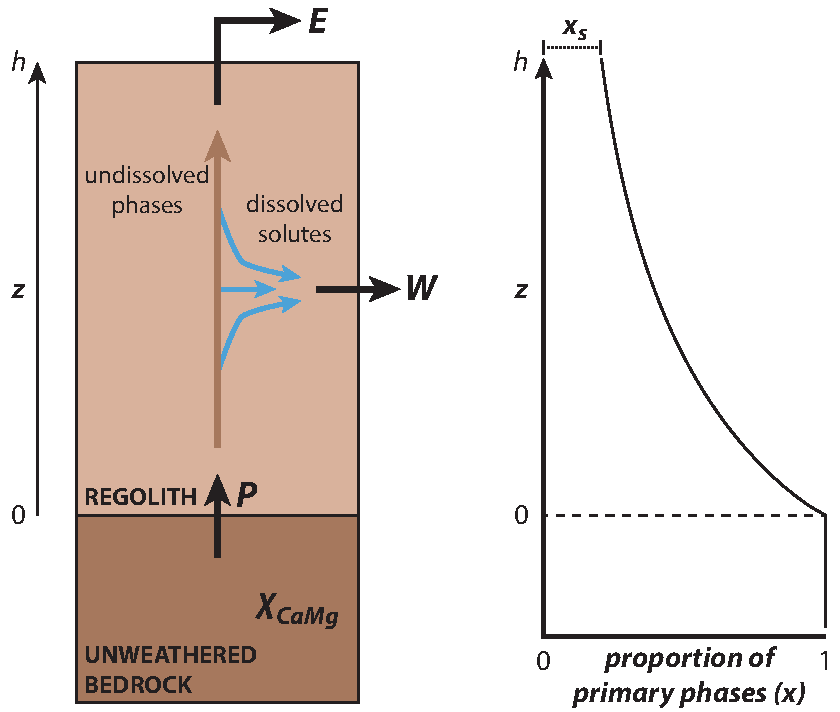
\includegraphics[width=.8\linewidth]{Figures/regolith_schematic.pdf}
\caption{Placeholder image of a frog with a long example legend to show justification setting.}
\label{fig:frog}
\end{figure}


\begin{SCfigure*}[\sidecaptionrelwidth][t]
\centering
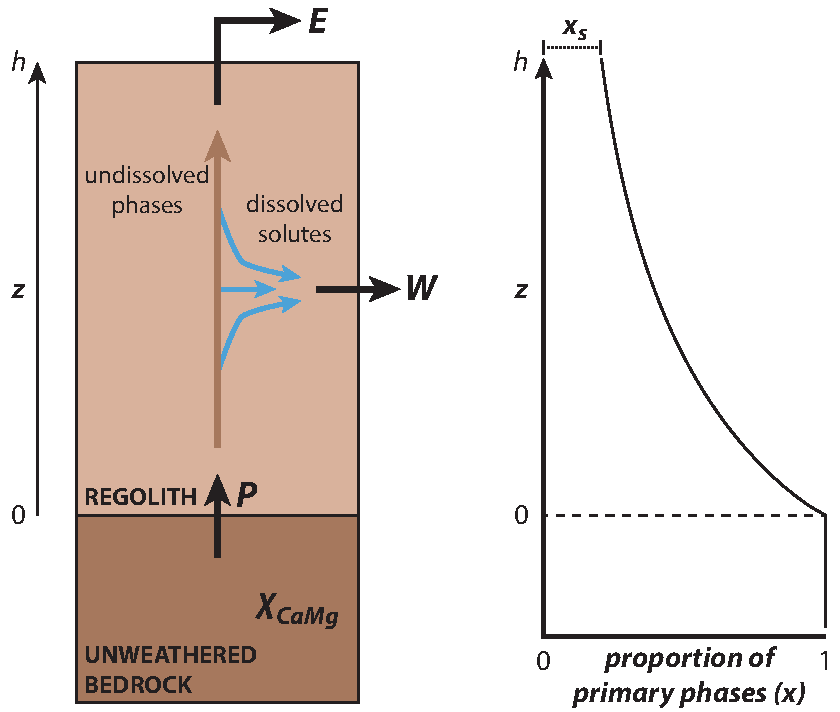
\includegraphics[width=11.4cm,height=11.4cm]{Figures/regolith_schematic.pdf}
\caption{This legend would be placed at the side of the figure, rather than below it.}\label{fig:side}
\end{SCfigure*}

\begin{figure*}[bt!]
\begin{align*}
(x+y)^3&=(x+y)(x+y)^2\\
       &=(x+y)(x^2+2xy+y^2) \numberthis \label{eqn:example} \\
       &=x^3+3x^2y+3xy^3+x^3. 
\end{align*}
\end{figure*}


\begin{table}%[tbhp]
\centering
\caption{Comparison of the fitted potential energy surfaces and ab initio benchmark electronic energy calculations}
\begin{tabular}{lrrr}
Species & CBS & CV & G3 \\
\midrule
1. Acetaldehyde & 0.0 & 0.0 & 0.0 \\
2. Vinyl alcohol & 9.1 & 9.6 & 13.5 \\
3. Hydroxyethylidene & 50.8 & 51.2 & 54.0\\
\bottomrule
\end{tabular}

\addtabletext{nomenclature for the TSs refers to the numbered species in the table.}
\end{table}

\matmethods{Please describe your materials and methods here. This can be more than one paragraph, and may contain subsections and equations as required. Authors should include a statement in the methods section describing how readers will be able to access the data in the paper. 

\subsection*{Subsection for Method}
Example text for subsection.
}

\showmatmethods{} % Display the Materials and Methods section

\acknow{Collaborative research between NLS-H and YG was initially supported by a grant from the France-Berkeley Fund. FAM and NLS-H gratefully acknowledge support through NSF FRES grants \#1926001 and \#1925990. We thank Alec Brenner, Sam Lo Bianco, Mariana Lin, and Judy Pu for their data compilation contributions to the paleoshoreline reconstructions. The GEOCLIM code associated with this study is openly available: \url{https://github.com/piermafrost/GEOCLIM-dynsoil-steady-state}}

\showacknow{} % Display the acknowledgments section

% Bibliography
\bibliography{References}

\end{document}
